\section{Fundamental Of Forward Converter}
The Forward Converter is a widely used topology in power electronics for medium-power applications (typically up to 200W). It provides isolated DC-DC conversion , making it suitable for applications requiring safety, noise immunity, and voltage regulation. Below is an explanation of its basic operation , key components , and important concepts like duty cycle , input/output voltage relationship , and efficiency .
\subsection{Basic Operation and Working Principle}
The forward converter operates by transferring energy from the input to the output through a transformer during the switch-on phase of the main switch (MOSFET). During the switch-off phase , the transformer resets, and the output inductor continues to supply current to the load. Here's a step-by-step breakdown:
\subsubsection*{Switch-On Phase}
When the MOSFET (main switch) is turned on:
\begin{itemize}
    \item Current flows through the primary winding of the transformer.
    \item Energy is transferred to the secondary winding, and the diode ($ D_1 $) conducts.
    \item The output inductor ($ L_f $) stores energy and supplies current to the load.
\end{itemize}
\begin{figure}[h!]
    \centering
    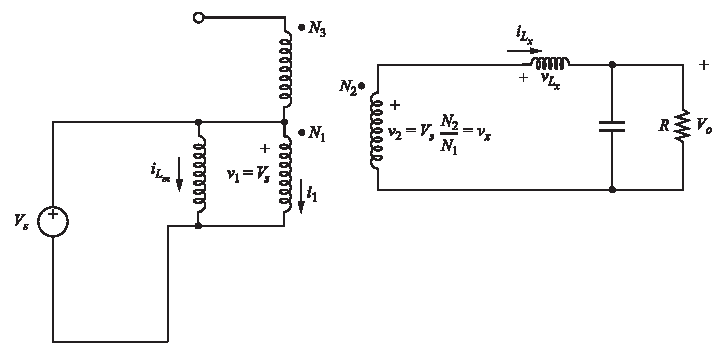
\includegraphics[width=0.7\linewidth]{Pictures/Images/2.pdf}
    \caption{\textcolor{blue}{\textit{\footnotesize Circuit for switch closed}}}
\end{figure}
\subsubsection*{Switch-Off Phase}
When the MOSFET turns off:
\begin{itemize}
    \item The transformer stops transferring energy, and the reset winding (or active clamp) resets the transformer core to prevent saturation.
    \item The energy stored in the output inductor ($ L_f $) continues to supply current to the load through the freewheeling diode ($ D_2 $).
\end{itemize}
This process repeats at a high switching frequency, ensuring continuous power delivery to the load.
\newpage
\begin{figure}[h!]
    \centering
    
\includegraphics[width=0.7\linewidth]{Pictures/Images/3.pdf}
    \caption{\textcolor{blue}{\textit{\footnotesize Circuit for switch
open}}}
\end{figure}
\subsection{Key Components}

The forward converter consists of several critical components that work together to achieve efficient and isolated power conversion:

\begin{itemize}
    \item \textbf{Transformer}: Provides \textbf{galvanic isolation} between the input and output. Steps down the input voltage to the desired output voltage based on the turns ratio ($ N_p : N_s $). Includes a \textbf{reset winding} or active clamp to reset the transformer core during the switch-off phase.
    \item \textbf{MOSFET}: Acts as the main switch to control energy transfer to the transformer. Operates at high frequencies to enable compact design.
    \item \textbf{Output Inductor ($ L_f $)}: Smooths the output current and ensures \textbf{Continuous Conduction Mode (CCM)}. Stores energy during the switch-on phase and releases it during the switch-off phase.
    \item \textbf{Output Capacitor ($ C_{out} $)}: Filters the output voltage to reduce ripple and provide a stable DC output.
    \item \textbf{Diodes}:
    \begin{itemize}
        \item $ D_1 $: Rectifies the secondary winding voltage during the switch-on phase.
        \item $ D_2 $: Freewheeling diode that maintains current flow to the load during the switch-off phase.
    \end{itemize}
    \item \textbf{Reset Mechanism}: A reset winding or active clamp circuit resets the transformer core to prevent saturation.
\end{itemize}
\subsection{Duty Cycle, Input/Output Voltage Relationship, and Efficiency}

\subsubsection*{Duty Cycle ($ D $)}
The duty cycle determines the fraction of time the MOSFET is on during each switching cycle. For a forward converter, the duty cycle is limited to:
$$
D < 0.5
$$
to allow sufficient time for the transformer core to reset during the switch-off phase.

\subsubsection*{Input/Output Voltage Relationship}
The relationship between the input voltage ($ V_{in} $), output voltage ($ V_{out} $), and transformer turns ratio ($ N_p : N_s $) is given by:
$$
V_{out} = V_{in} \cdot \frac{N_s}{N_p} \cdot D
$$
Where:
\begin{itemize}
    \item $ N_p $: Number of turns in the primary winding.
    \item $ N_s $: Number of turns in the secondary winding.
    \item $ D $: Duty cycle.
\end{itemize}

\subsubsection*{Efficiency}
The efficiency of the forward converter is determined by minimizing losses in the following areas:
\begin{itemize}
    \item \textbf{Switching Losses}: Occur due to the MOSFET turning on and off at high frequencies.
    \item \textbf{Conduction Losses}: Caused by the resistance of the MOSFET, diodes, and windings.
    \item \textbf{Core Losses}: Result from hysteresis and eddy currents in the transformer core.
    \item \textbf{Output Ripple Losses}: Due to filtering components (inductor and capacitor).
\end{itemize}